% !TEX root=main.tex

\section{Control system design}

\subsection{PD controller design}

We want to design a limited PD controller with the transfer function

\begin{equation}
    H_{pd}(s) = K_{pd}\frac{1+T_ds}{1+T_fs} \label{eq:H_pd}
\end{equation}

to control the heading $\psi$ of the ship, by setting the rudder angle $\delta$. We want the cross frequency and phase margin of the open loop system to be $0.10\si{\radian\per\second}$ and $50$ degrees respectively. We also want the time constant $T_d$ to equal the time constant of the system. In order to choose $K_{pd}$, $T_d$ and $T_f$ we first find the transfer function of the open loop system

\begin{equation}
    H_{sys}(s) = H_{pd}(s) \cdot H_{ship}(s) = KK_{pd}\frac{1+T_ds}{s(Ts+1)(T_fs+1)} \label{eq:H_sys}
\end{equation}

As we want $T_d$ to equal the time constant of the model we set $T_d = T = 86.5246 \si{\second}$. Next we use that the phase margin of a system is equal to $\angle H(j\omega_c) + 180 \si{\degree}$.

\begin{subequations}
    \begin{align}
        \angle H_{sys}(j\omega_c) + 180 \si{\degree} &= 50 \si{\degree} \\
        \angle \frac{KK_{pd}}{(j\omega_c)^2T_f+j\omega_c} &= -130 \si{\degree}\\
        \angle KK_{pd} - \angle ((j\omega_c)^2T_f+j\omega_c) &= -130 \si{\degree} \\
        \angle ((j\omega_c)^2T_f+j\omega_c) &= -130\si{\degree} \\
        \tan^{-1}\frac{\omega_c}{\omega_c^2T_f} &= 50 \si{\degree} \\
        T_f &= \frac{1}{ \omega_c \tan (50 \si{\degree}) } \\
        T_f &= 8.3910 \si{\second} \label{eq:T_f}
    \end{align}
\end{subequations}

Last we find $K_{pd}$ by using the definition of the cross frequency: $|H(j\omega_c)| = 1$. This yields

\begin{subequations}
    \begin{align}
        |H_{sys}(j\omega_c) &= 1 \\
        |H_{sys}^2(j\omega_c) &= 1^2 \\
        \left | \frac{KK_{pd}}{s^2T_f+s} \right |^2 &= 1 \\
        \frac{(KK_{pd})^2}{(\omega_c^2 T_f)^2 + \omega_c^2} &= 1 \\
        K_{pd} &= \frac{\sqrt{(\omega_c^2 T_f)^2} + \omega_c^2}{K} \label{eq:K_pd(T_f)}
    \end{align}
\end{subequations}

Inserting \cref{eq:T_f} into \cref{eq:K_pd(T_f)} yields a $K_{pd} = 0.7494$. The controller was implemented in Simulink as seen in \cref{fig:pd}.

\begin{figure}
    \centering
    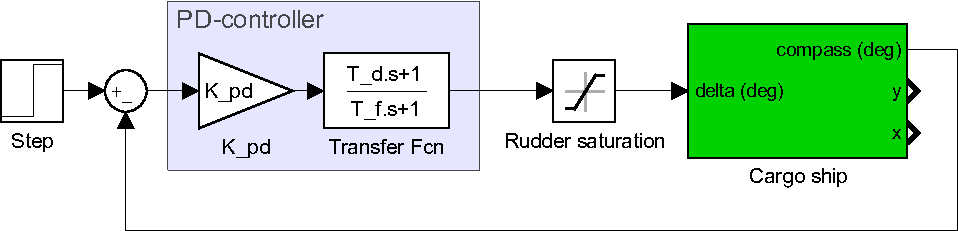
\includegraphics[width=\textwidth]{images/oppg3/a_pd-loop.pdf}
    \caption{Simulink implementation of the PD-controller.}
    \label{fig:pd}
\end{figure}

\subsection{Performance without disturbances}

As we can see in \cref{fig:step_no_dist} the controller does a good job when there are no disturbances. The ship gets close to reference $\psi_r$ of $30\si{\degree}$ about 2 minutes, and the rudder angle is relatively constant over time.

\begin{figure}
    \centering
    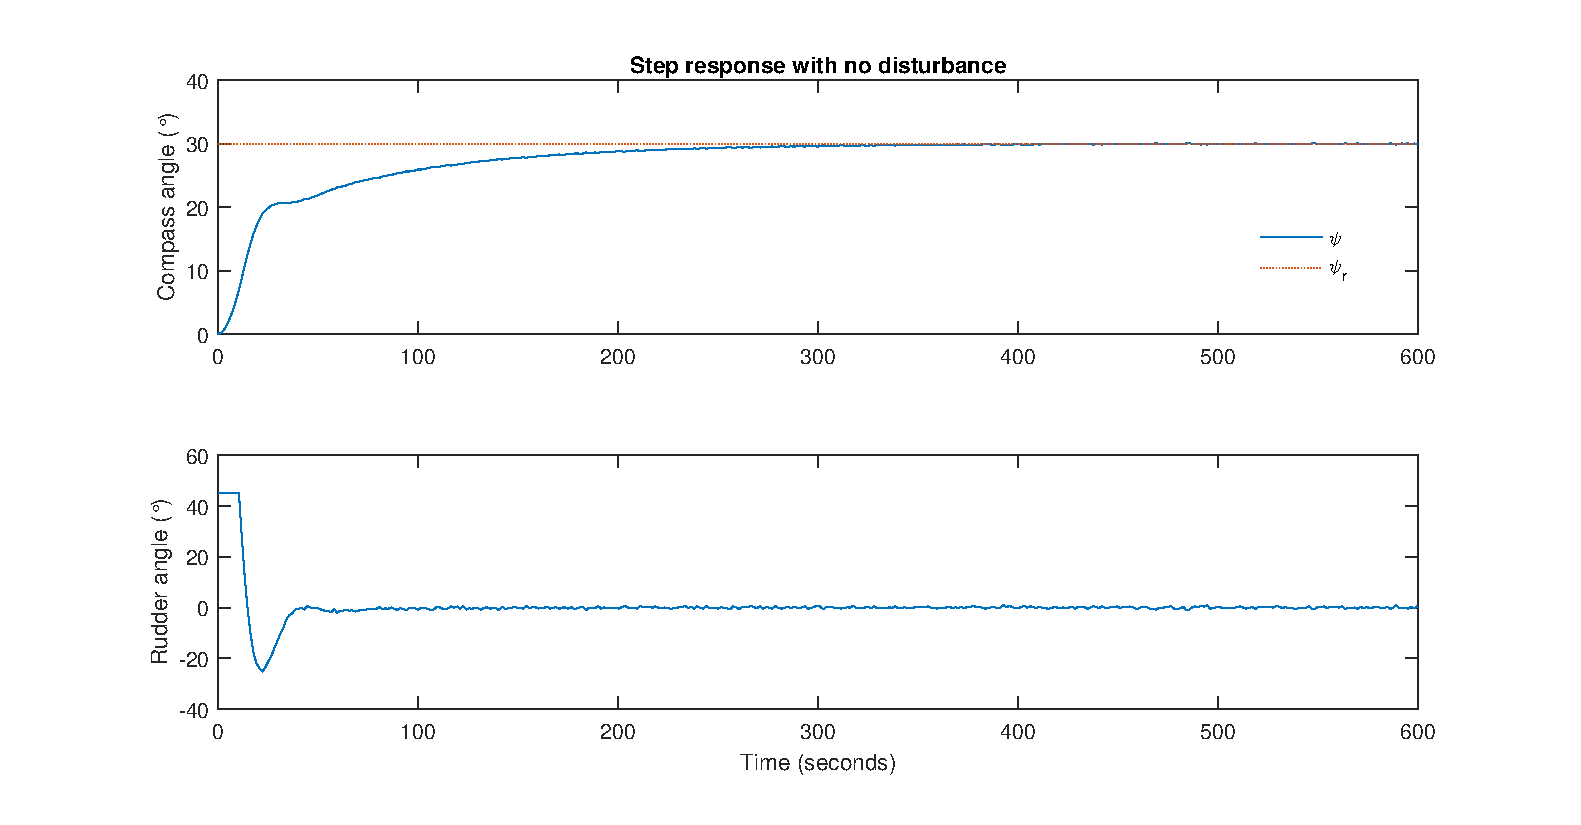
\includegraphics[width=\textwidth]{images/oppg3/stepresp_no_disturbance.eps}
    \caption{Step response of the controller without any disturances.}
    \label{fig:step_no_dist}
\end{figure}

\subsection{Performance with a current disturbance}

In \cref{fig:step_current_dist} we see the response of the controller with current disturbance. As we can see the controller is unable to counteract the constant disturbance of the current, which leads to a large constant deviation from the setpoint.

\begin{figure}
    \centering
    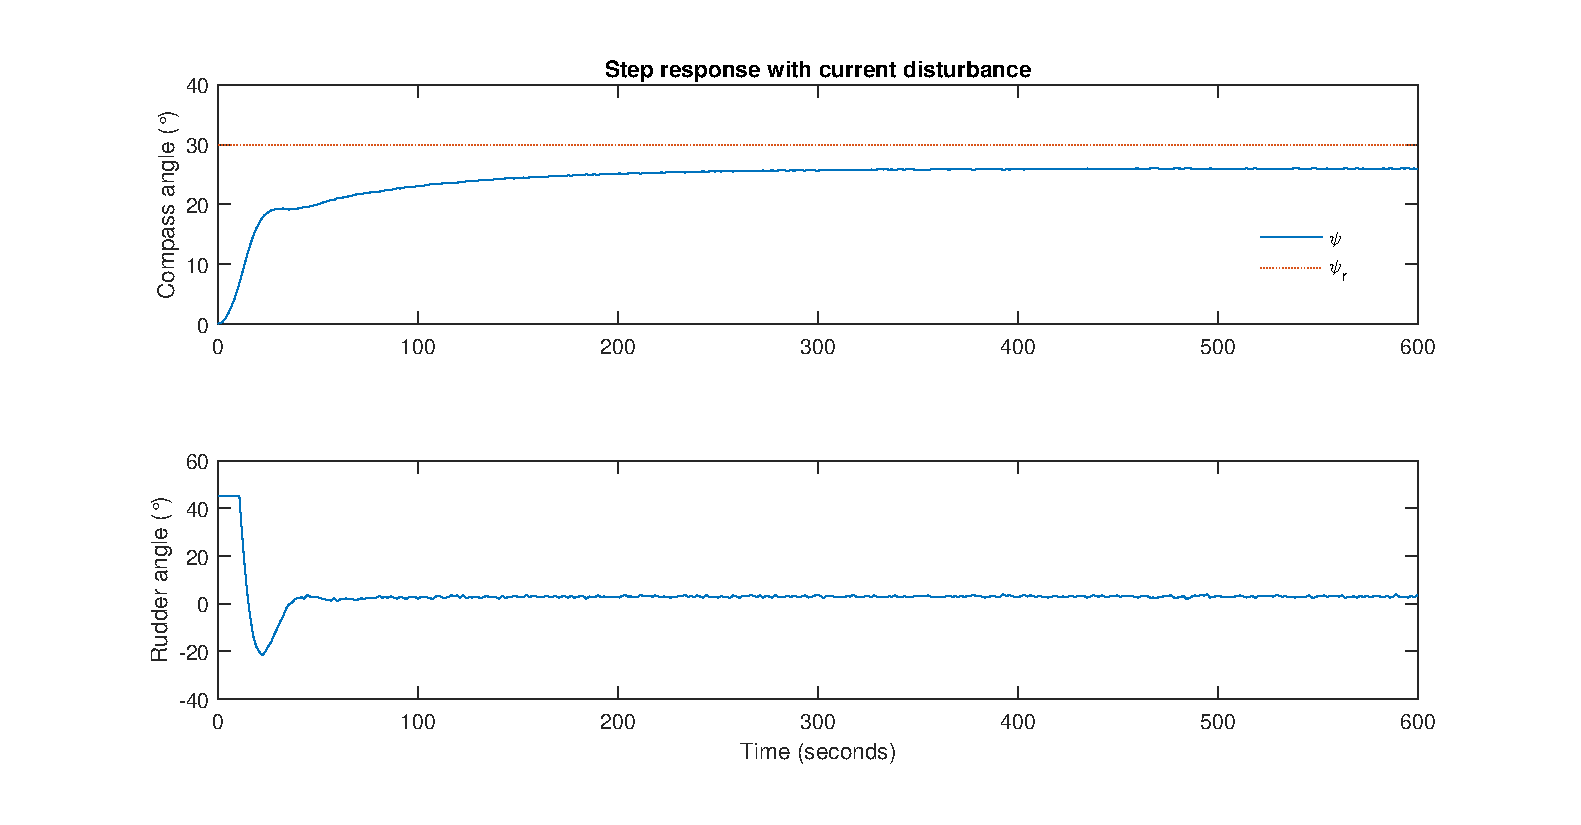
\includegraphics[width=\textwidth]{images/oppg3/stepresp_current_disturbance.eps}
    \caption{Step response of the controller with current disturbance.}
    \label{fig:step_current_dist}
\end{figure}

\subsection{Performance with wave disturbance}

When we apply wave current (and turn off current disturbance), we see in \cref{fig:step_wave_dist} that the controller does its best to remove the noise but is unable to do much about it. In its attempt to remove the noise it applies a lot of rudder input, which if the boat were real would stress the physical system.

\begin{figure}
    \centering
    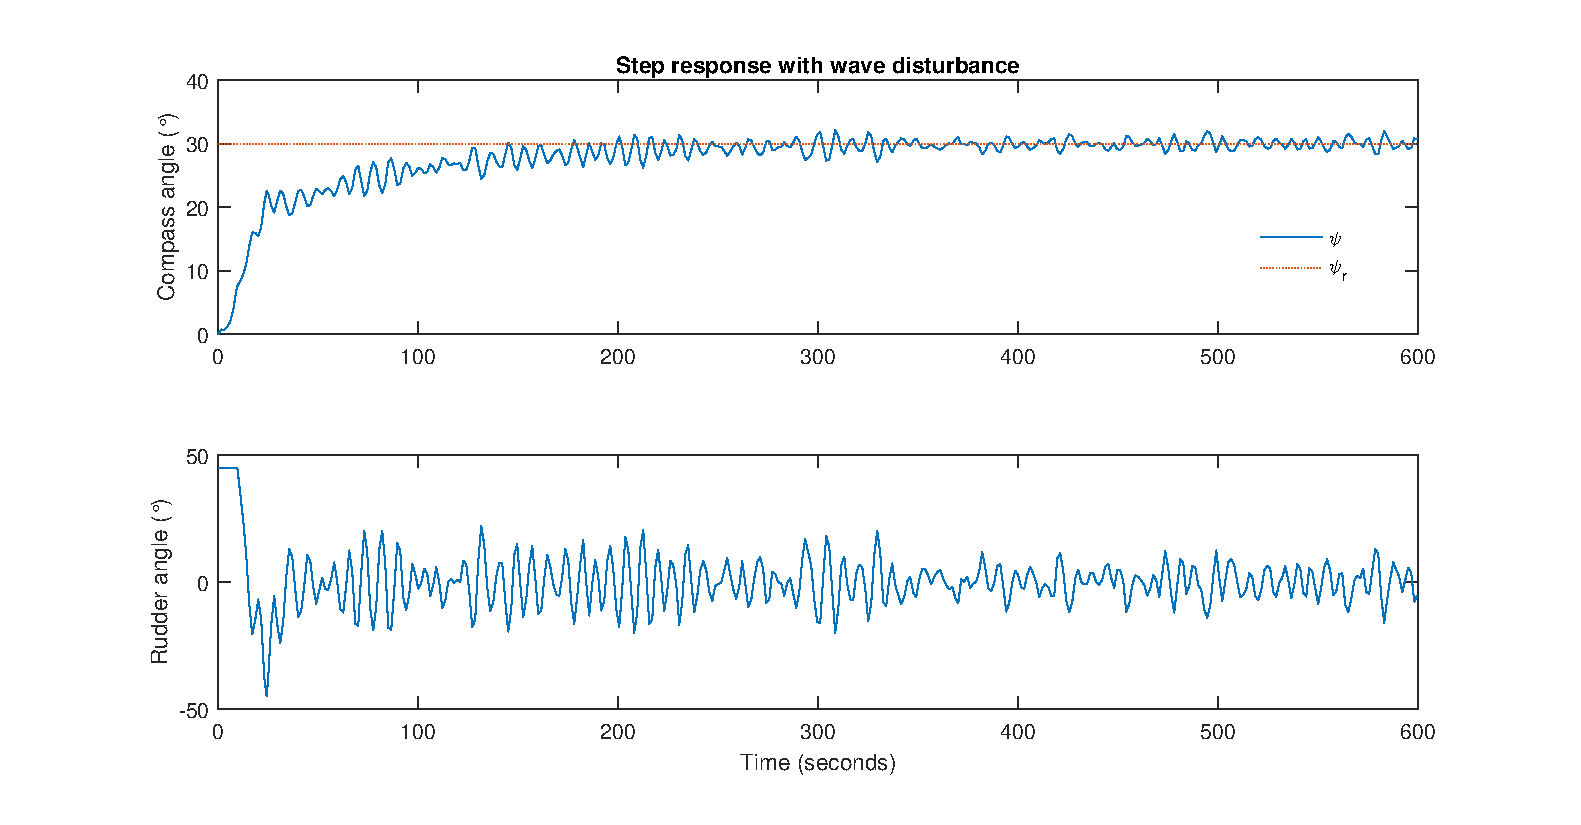
\includegraphics[width=\textwidth]{images/oppg3/stepresp_wave_disturbance.eps}
    \caption{Step response of the controller with wave disturbance.}
    \label{fig:step_wave_dist}
\end{figure}
